\cotefile{156-4}
\scanpage{66}\mspage{65}
This follows from \deleted{\uline{C}4 and} corollary 1 and from the

\uline{Lemma} For $F$ to be of finite type\inserted{(resp. finite)} it is necessary and sufficient that a) the $F_i$ be so and b) All the $F_i$ except a finite number are $\varnothing$.

Notations $\pi_0(F)$ (NB If $F\leq G$ we have $\pi_0(F)\longrightarrow\pi_0(G)$\deleted{\unsure{)}}, and transitivity) $\pi_0(M)$, $\pi_0^{\substack{\deleted{\unsure{\mathrm{cat}|\mathrm{act}}}\\!}}(\unsure{.}\mathcal F)$. (\unsure{Caution}, the $\pi_0^{\unsure{\underset{\circ}{d}|!}}(\mathcal F)$ is not the $\pi_0(F,\leq)$, but the $\pi_0$ ``taking account \unsure{of the|of the} Sup''. If
% The tuple and its two interlinear glosses are reproduced together with their drawn pointers.
\figure{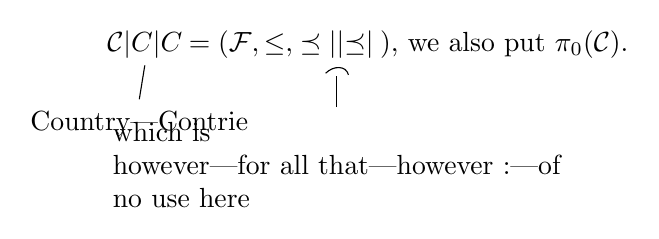
\begin{tikzpicture}[every node/.style={inner sep=1pt}]
  \node[anchor=base west] (initial) at (0,0) {$\unsure{\mathcal C|\mathscr C|C}$};
  \node[anchor=base west] (prefix) at (initial.base east) {$=(\mathcal F,\leq,$};
  \node[anchor=base west] (relation) at (prefix.base east) {$\unsure{\preceq|\leqslant|\deleted{\preceq}|\deleted{\leqslant}}$};
  \node[anchor=base west] (rest) at (relation.base east) {$)$, we also put $\pi_0(\mathcal C)$.};
  \draw[thin] (initial.south) ++(0,-0.05) -- ++(-0.07,-0.43);
  \path (initial.south) ++(-0.07,-0.60)
    node[anchor=north] {\unsure{Country|Contrie}};
  \draw[thin] (relation.south) ++(0,-0.58) -- ++(0,0.40);
  \draw[thin] (relation.south) ++(-0.14,-0.15)
    .. controls +(0.10,0.10) and +(-0.03,0.12) .. ++(0.29,-0.02);
  \path (relation.south) ++(0,-0.73)
    node[anchor=north,align=left] {which is\\\unsure{however|for\deleted{ all that}|\deleted{however}} \unsure{:|of}\\no use here};
\end{tikzpicture}}

Strengthened axiom

\uuline{C4 bis} For every $(F_i)_i\in\prod\mathcal F_i$, $\deleted{\exists\mathcal F}$ $\exists F\in\mathcal F$ such that $F\mid M_i=\unsure{F_i|\deleted{\mathcal F}F_i}$ for $i\vdash I$,

\uline{Residual \unsure{country|Contrie}} \uline{Support} \uline{and} \uline{cosupport}

Let $\deleted{\unsure{(F_i)\in\mathcal F|(H_i)\in\mathcal F}}$ $\Phi\subset\mathcal F$ be a set of
% The inserted H_i is connected to the position after figures by a long oblique stroke.
\figure{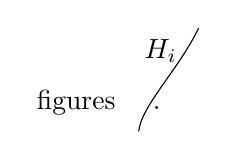
\begin{tikzpicture}[x=1cm,y=1cm]
  \node[anchor=base east] at (0,0) {figures};
  \node[anchor=base] at (0.45,0.65) {\inserted{$H_i$}};
  \draw (0.17,-0.28) .. controls (0.20,0.04) and (0.68,0.51) .. (0.93,1.03);
  \node[anchor=base] at (0.40,0) {.};
\end{tikzpicture}}
\deleted{We shall put} Let $F$ be a figure. For \deleted{Cosupport $\Phi$} $F$ to be \unsure{disjoint|disjoint} from all the $H_i$, it is necessary and sufficient that this be the case for all the \unsure{strata} of $F$ (because of C3). \deleted{Put} Put
